\documentclass{article}

\usepackage{amsmath,amsthm,amsfonts,amssymb,bm}
\addtolength{\textheight}{5.0cm}
\addtolength{\voffset}{-3.5cm}
\addtolength{\hoffset}{-2.5cm}
\addtolength{\textwidth}{4.0cm}

\allowdisplaybreaks

\usepackage{subeqnarray}
\usepackage{mathrsfs}
\usepackage[usenames,dvipsnames]{color}
\usepackage{url}
\usepackage{ulem}
\usepackage{indentfirst}
%\usepackage{textcomp}
%\usepackage{graphics}
\usepackage{graphicx}
\usepackage[hang,small,bf]{caption}
\setlength{\captionmargin}{50pt}

%includeonly{}


\graphicspath{{Figures/}{Figures/CPL/}{Figures/DE/}{Figures/P/}}


%\usepackage{tikz}
%\usetikzlibrary{mindmap,trees}

\begin{document}
\title{Power Spctrum \& Its Evolution}
\author{MA Lei}
\maketitle


%%%%%%%%%%%%%%%%%%%%%%%%%%%%%%%%%%%%%%%%%%%%%%%%%%%%%%%%%
%%%%%%%%%%%%%%%%%%%%%%%%%%%%%%%%%%%%%%%%%%%%%%%%%%%%%%%
%%%%%%%%%%%%%%%%%%%%%%%%%%%%%%%%%%%%%%%%%%%%%%%%%%%%%%%%
%%%%%%%%%%%%%%%%%%%%%%%%%%%%%%%%%%%%%%%%%%%%%%%%%%%%%%%
%%%%%%%%%%%%%%%%%%%%%%%%%%%%%%%%%%%%%%%%%%%%%%%%%%%%%%%



\newpage    %It is weird that this command solve the problem that the figure goes between the double line and the text.
\hrule\vspace{1pt}\hrule
\begin{center}
\mbox{{\bf XXXX}} \\
\vspace{0.5em}
\mbox{{XXXX}}
\end{center}
\hrule



\section{Work}

\subsection{Repeat Fernando's work}

\subsubsection{Preparing}

To get the figures in their paper, a figure that describes the relation between growth and the wavenumber $k$ (Growth VS $k$) should be calculated.

\begin{itemize}
\item
Any growth factor can be calculated using the method in previous section.

\item
The next work is to calculate the Hubble distance (because this determines when do the perturbations come into the horizon) of scale factor.

Hubble distance is 
\footnote{
For more details check the {\it Cosmology Projects} notebook}
\begin{equation}
d_H=\int^{a}_{0}{ \frac{\mathrm d a'}{a'^2H(a')} }
\end{equation}

Then we can use the current $d_H(a(t_0))$ and MD approximation of $H(a(t))$ (since we will only cal. the MD evolution of the perturbations.) 
\footnote{
There are many things to be considered. 
\begin{itemize}
\item 
Different models might give different evolution of Hubble distance. And what is knotty is that the models might give different current value of Hubble distance when given a suitable set of parameters (because one might focus on other things to fit the parameters). (???) 

\end{itemize}}

$H(a(t))$ can be simplified into 
\begin{equation}
H(a)=H_0 (\Omega_{M0}a^{-3}+\Omega_{DE0}a^{-3(1+w)})
\end{equation}
according the fact that current observation shows the universe is filled with 73\% dark energy and 27\% matter (mostly dark matter).

\end{itemize}


\subsubsection{$\Lambda$CDM}

Parameters
\begin{eqnarray*}
w=-1;\Omega _{\text{DE0}}=0.734;\Omega _{\text{k0}}=0;\Omega _{\text{m0}}=0.1334\left/\left(0.71^2\right)\right.;\Omega _{\text{r0}}=8.09*10^{-5};
\end{eqnarray*}

Hubble distance:
\begin{figure}[!htbp]
\centering
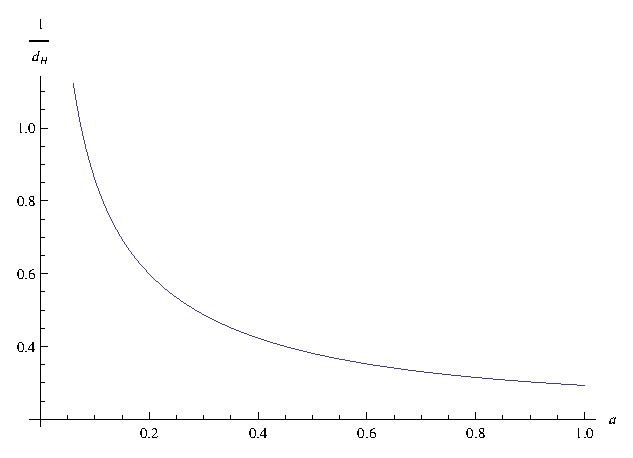
\includegraphics[width=400pt]{P_LCDM_HubbleDistance.eps}
\caption{$\frac{1}{d_H}$ vs $a$}
\end{figure}

growth factor:
\begin{figure}[!htbp]
\centering
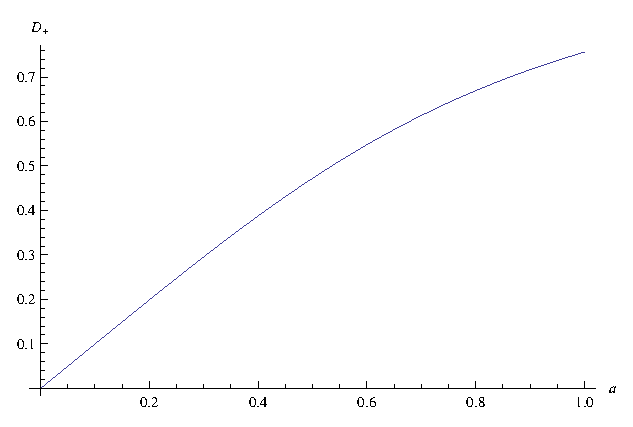
\includegraphics[width=400pt]{P_LCDM_Growth.eps}
\caption{growth factor}
\end{figure}

Growth vs $k$
\begin{figure}[!htbp]
\centering
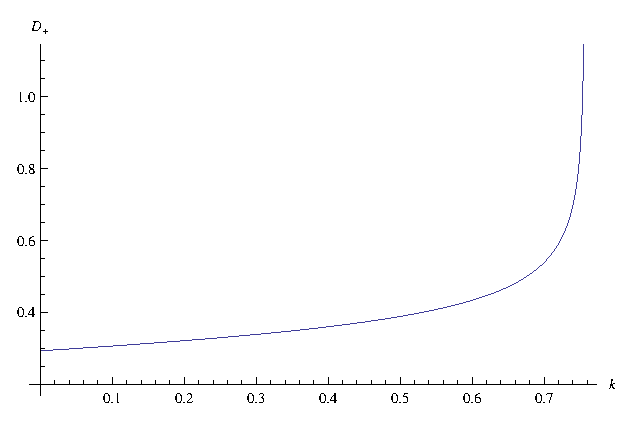
\includegraphics[width=400pt]{P_LCDM_GrowthVSk.eps}
\caption{Growth}
\end{figure}




\subsubsection{LCDM and Dark Energy}

Parameters are listed below.

\begin{eqnarray}
&\Omega _{\text{DE0}}=0.734;\Omega _{\text{k0}}=0;\Omega _{\text{m0}}=0.1334\left/\left(0.71^2\right)\right.;
\Omega _{\text{r0}}=8.09*10^{-5};
\\
&\Omega _{\text{m0},s}=1;\Omega _{\text{r0},s}=8.09*10^{-5};\\
&h=0.71;H_0=\frac{100 h}{300000};
\end{eqnarray}

Each color in the figures represents a model.
\vspace{2ex}
\begin{center}
\begin{tabular}{|c|c|}\hline
{\bf Color} & {\bf Model} \\\hline
Red & sCDM \\\hline
Orange & LCDM \\\hline
Yellow & $w=-0.25$ \\ \hline
Green &  $w=-0.5$ \\ \hline
Blue & $w=-0.75$ \\ \hline
\end{tabular}
\end{center}
\vspace{2ex}





\begin{figure}[!htbp]
\centering
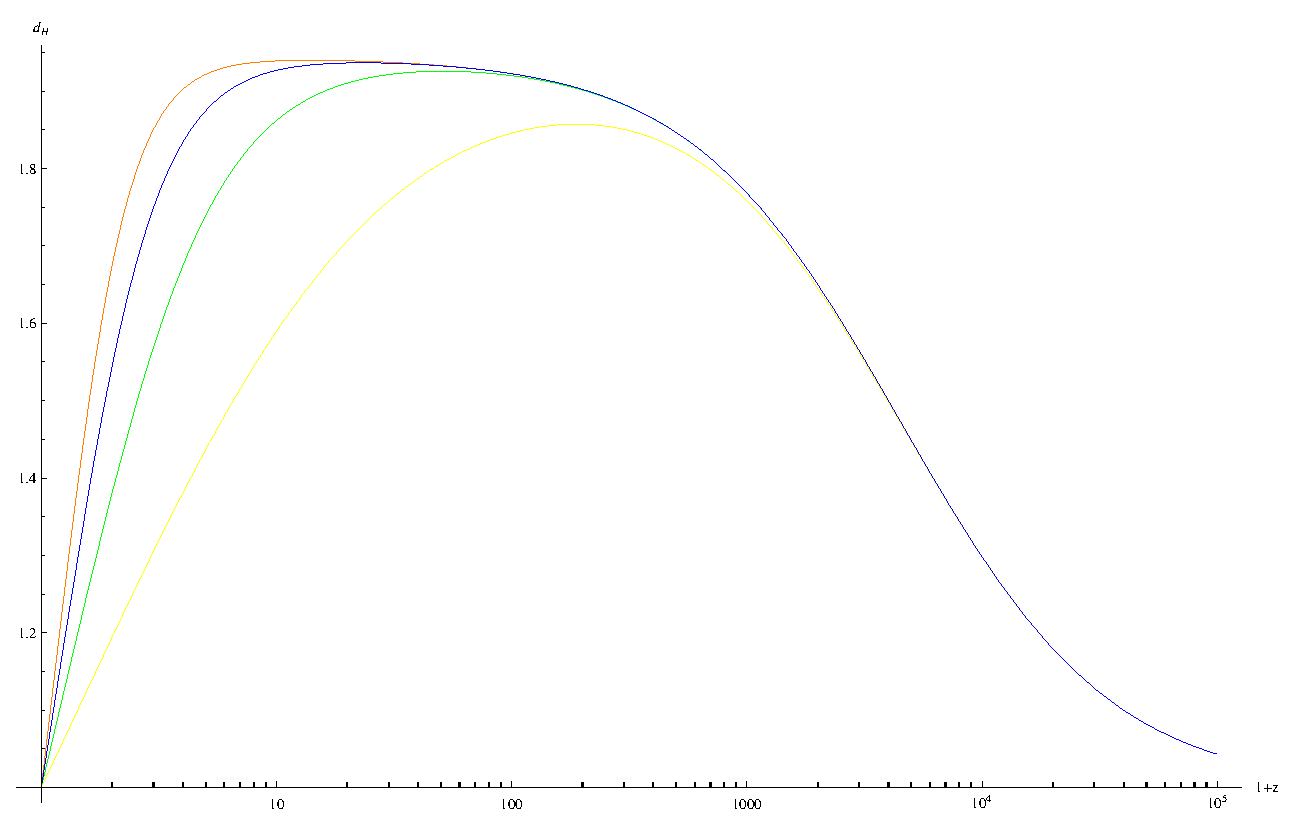
\includegraphics[width=400pt]{DE_HubbleDistances.eps} 
\caption{Hubble distances}\label{fig:DE_HubbleDistances}
\end{figure}


Figure \ref{fig:DE_HubbleDistances} shows the differences of the evolution of the Hubble distance. All the data are normalised with the inverse of sCDM's Hubble distance.
The shape of the lines can be explained by the fact that DE or Lambda only changes the background of the universe at late times after RD. The reason for the dropping down of the lines is that the Hubble functions should have the same value today ($1+z=1$). That is also the reason for the fact that they cross the same point at $1+z=1$. (Values of Hubble equations should converge at late times. So the part with $1+z<1$ is useless.)

Through figure \ref{fig:DE_HubbleDistances} the three DE models fall between LCDM and sCDM which should be a straight line of value 1. Since the EoS of three DE models are exactly between 0 and -1, this result is quite reasonable. This figure also shows that the DE model with $w=-0.25$ obviously deviates from LCDM at an early age of $z\sim 1000$, while other models deviate after about $z\sim 50$.






\begin{figure}[!htbp]
\centering
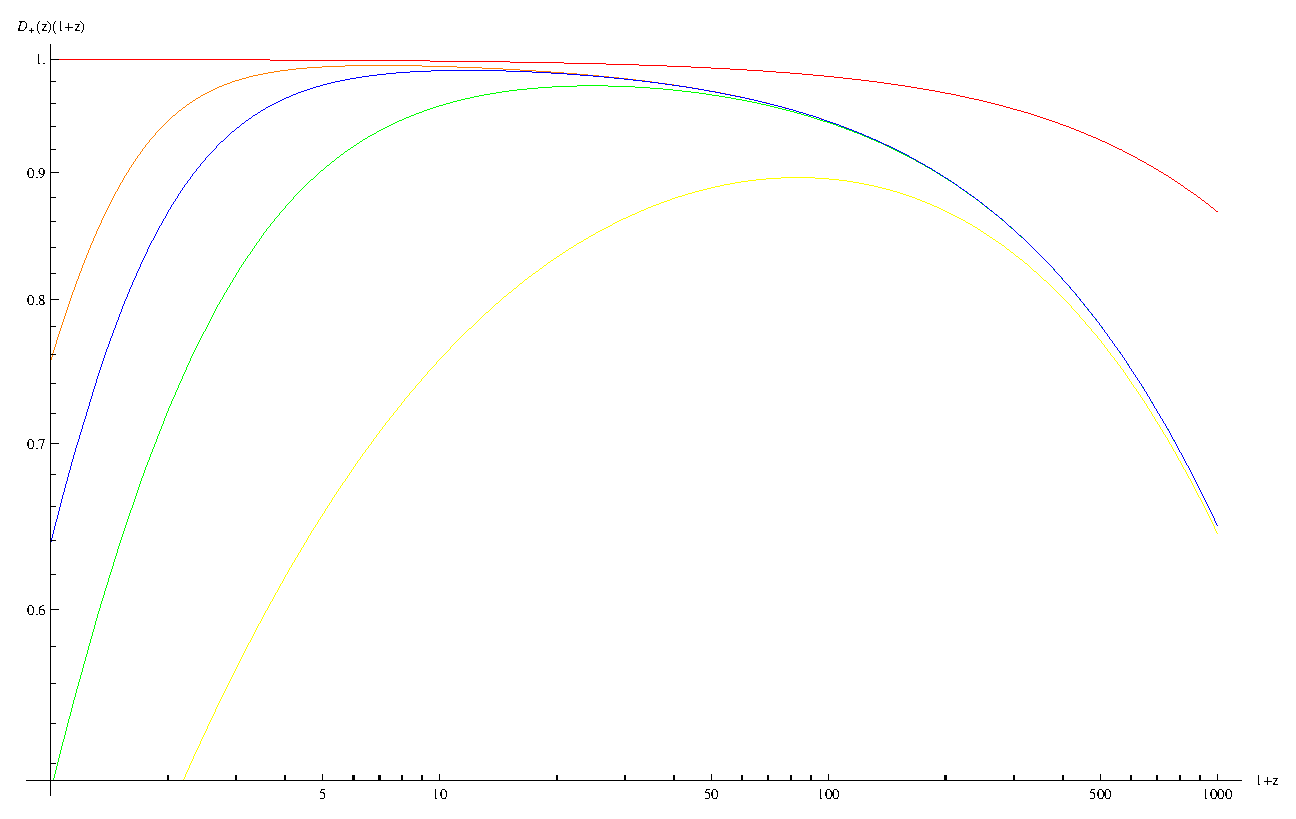
\includegraphics[width=400pt]{DE_GrowthFactors.eps} 
\caption{Growth factors vs $1+z$ of DE and $\Lambda$CDM}\label{fig:DE_GrowthFactors}
\end{figure}


Figure \ref{fig:DE_GrowthFactors} are the growth factors of the models. The going down lines are due to the late age effect of dark energy which suppresses the evolution of perturbations.

[{\color{red}\bf \it Why does the yellow line ($w=-0.25$) behave so strangely? Though we only use the part with $1+z$ larger than 1, it is hard to imagine it crossing LCDM (while other lines crossing nothing).}]






\begin{figure}[!htbp]
\centering
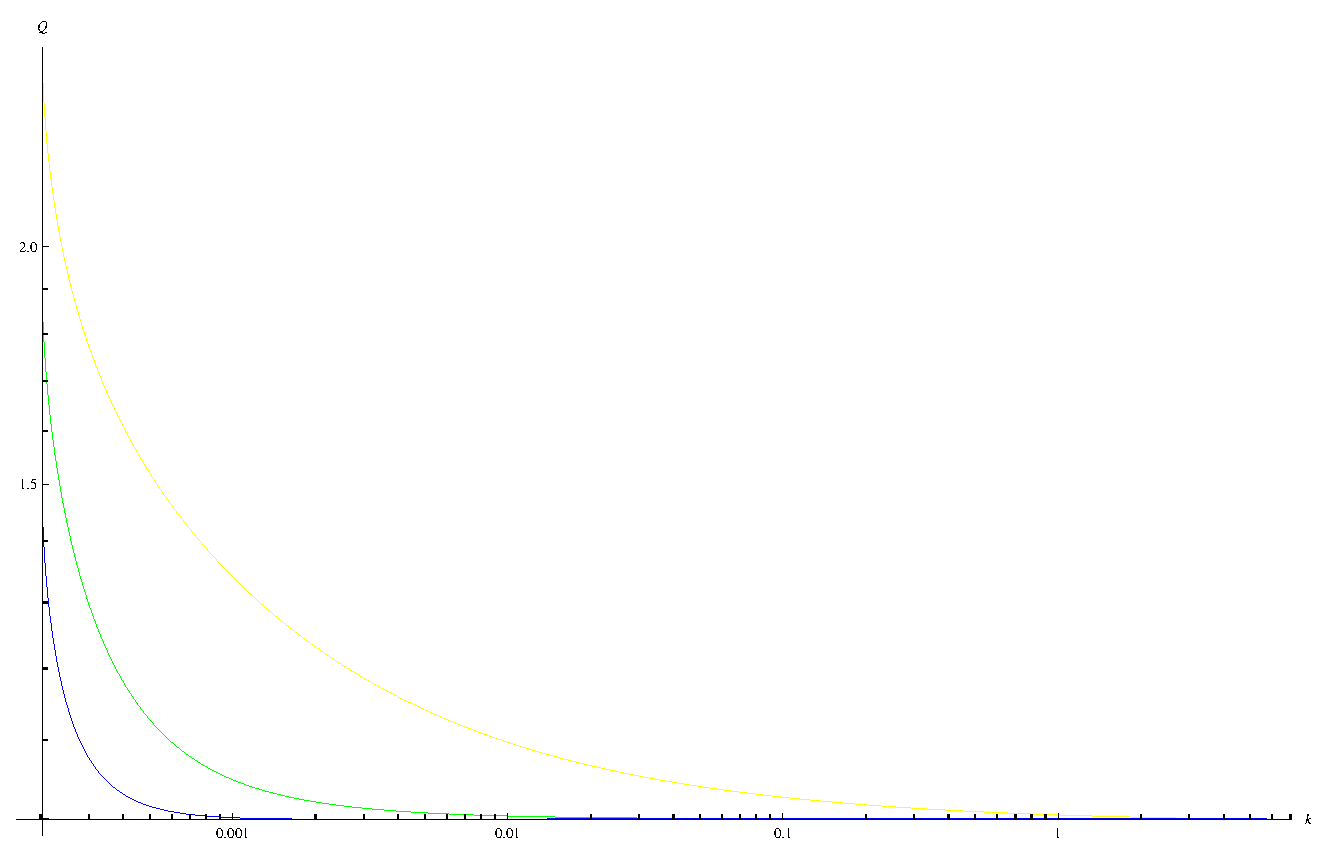
\includegraphics[width=400pt]{DE_QFactors.eps} 
\caption{Q factors}\label{fig:DE_QFactors}
\end{figure}



\begin{figure}[!htbp]
\centering
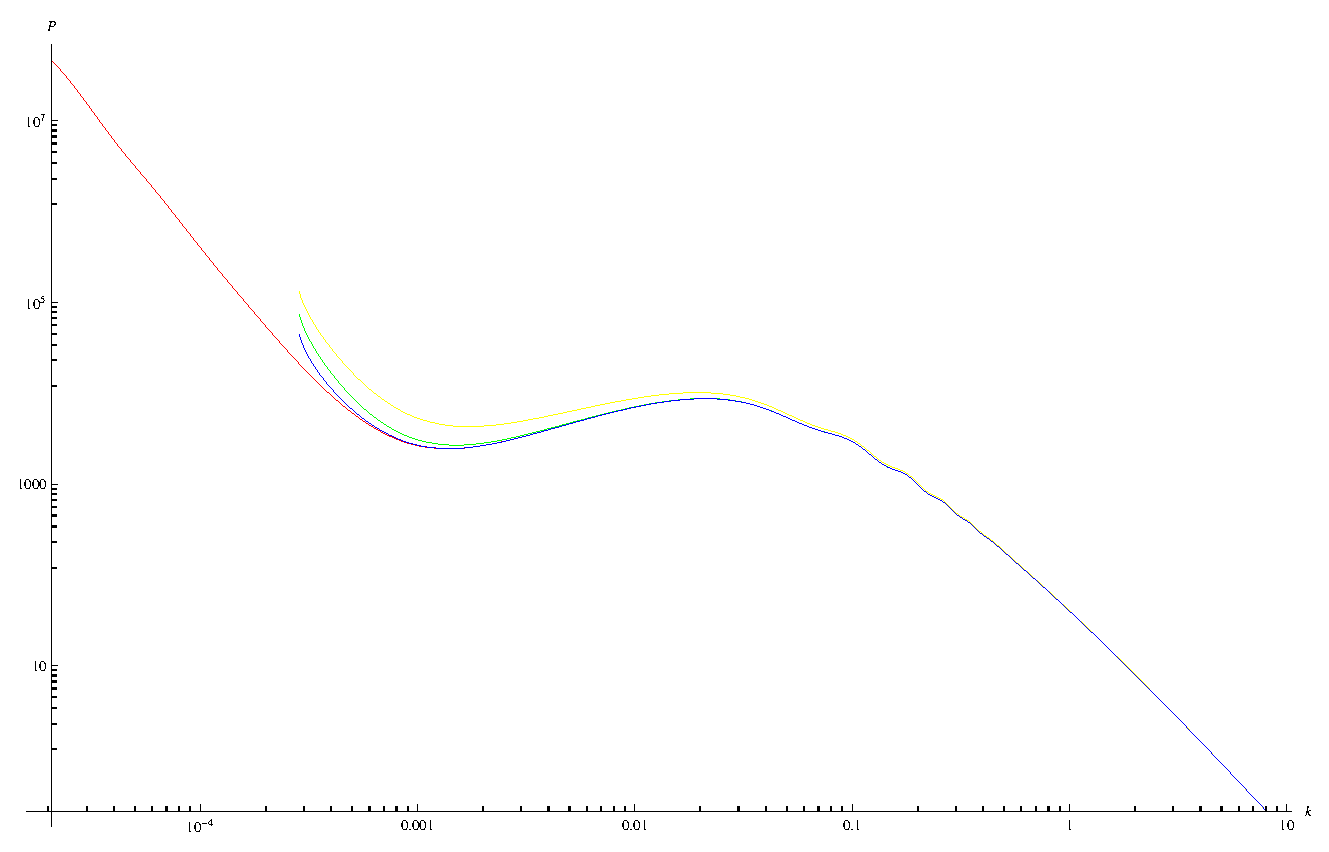
\includegraphics[width=400pt]{DE_PowerSpectrums.eps}
\caption{Power spectrum of LCDM and several DE models}\label{fig:DE_PowerSpectrums}
\end{figure}

\begin{figure}[!htbp]
\centering
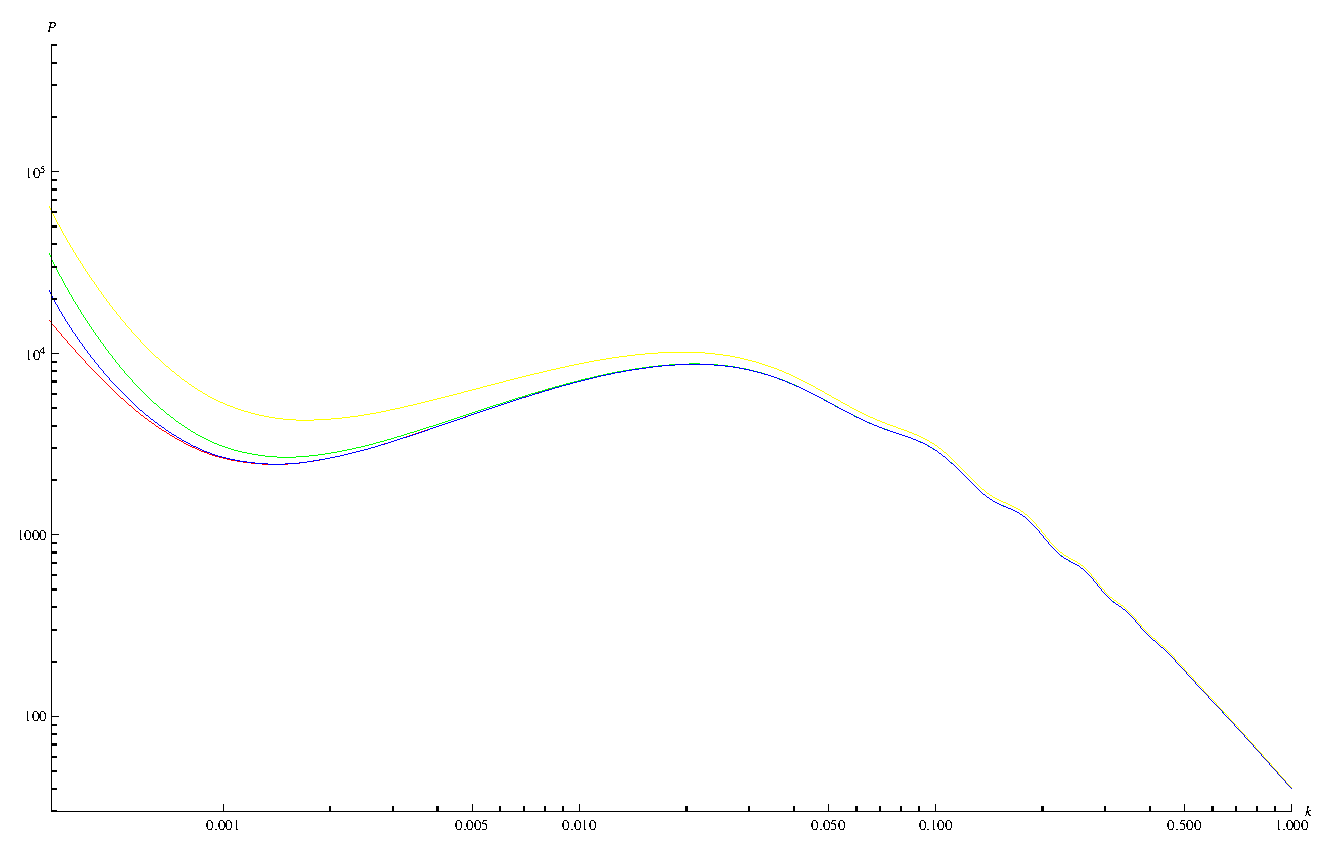
\includegraphics[width=400pt]{DE_PowerSpectrums_Cut.eps}
\caption{Power spectrum (within a range) of LCDM and several DE models}\label{fig:DE_PowerSpectrums_Cut}
\end{figure}



Figure \ref{fig:DE_PowerSpectrums} shows the power spectrums, which are generated by the standard LCDM model. The figure gives the lines the right trend when change the EoS, just as right as the Hubble distance.

One thing that is really annoying is that as the EoS becomes more and more close to LCDM, it is harder and harder to distinguish the DE models with LCDM models. The blue line is a good example for this statement.



These results supports the point that this method works well for these time independent EoS DE models and it can be show the differences of the models in between the time interval we are working on.











\subsection{CPL}


\subsubsection{What Is CPL Parameterisation?}

Notes in {\it Cosmology Project Notebook}.

The EoS here is $w=w_0+w_a(1-a)$.

\subsubsection{Generating Power Sepctrum}

The figures in this subsubsection follows the following rules unless exceptions are stated:
\begin{itemize}
\item
Red for sCDM;orange for LCDM;yellow for 

\end{itemize}

Parameters table (other parameters are exactly the same with the previous calculation):

\vspace{2ex}
\begin{center}
\begin{tabular}{|c|c|}\hline
{\bf Color} & {\bf Model} \\\hline
Red & sCDM \\\hline
Orange & LCDM \\\hline
Yellow & $w_a=-0.20$ \\ \hline
Green &  $w_a=-0.30$ \\ \hline
Blue & $w_a=-0.32$ \\ \hline
Cyan & $w_a=-0.34$ \\ \hline
Purple & $w_a=-0.44$ \\ \hline
\end{tabular}
\end{center}
\vspace{2ex}

In these CPL models, the parameters make sure that $w_0+w_a=-1$ in order to generate a background analogous to LCDM.

It should be made clear that the range of validity is around $10^{-4}<k<10$ or equivalently a range of $10^{-3}<a<1$.




\begin{figure}[!htbp]
\centering
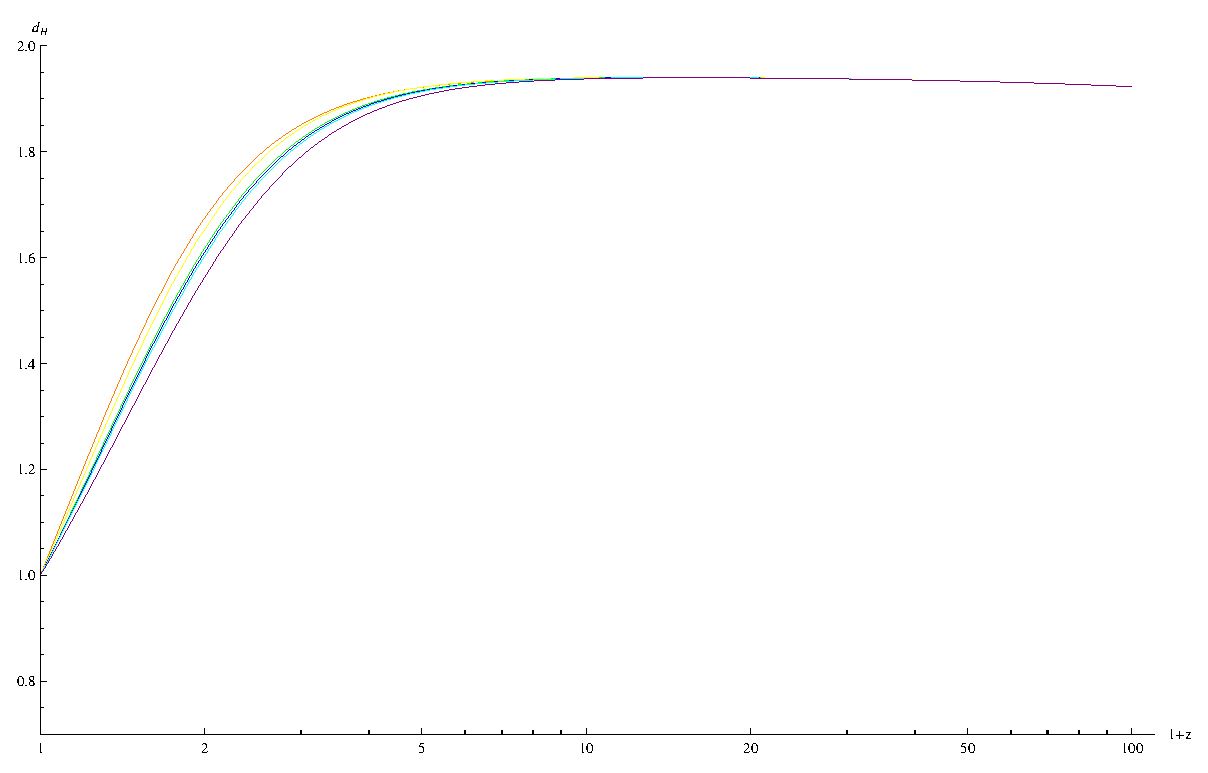
\includegraphics[width=400pt]{CPL_HubbleDistances.eps}
\caption{The Hubble distance of different models including sCDM, LCDM and five other CPL parameterised dark energy model}\label{fig:CPL_HubbleDistances}
\end{figure}

Figure \ref{fig:CPL_HubbleDistances}  shows the Hubble distances. The $1+z<1$ part is also useless so I cut them off. The smaller the EoS is, the larger the Hubble distance is during late ages. The parameters chosen here are all fits to LCDM well. So the difference between between them is small. However the differences are large enough to be noticed.



\begin{figure}[!htbp]
\centering
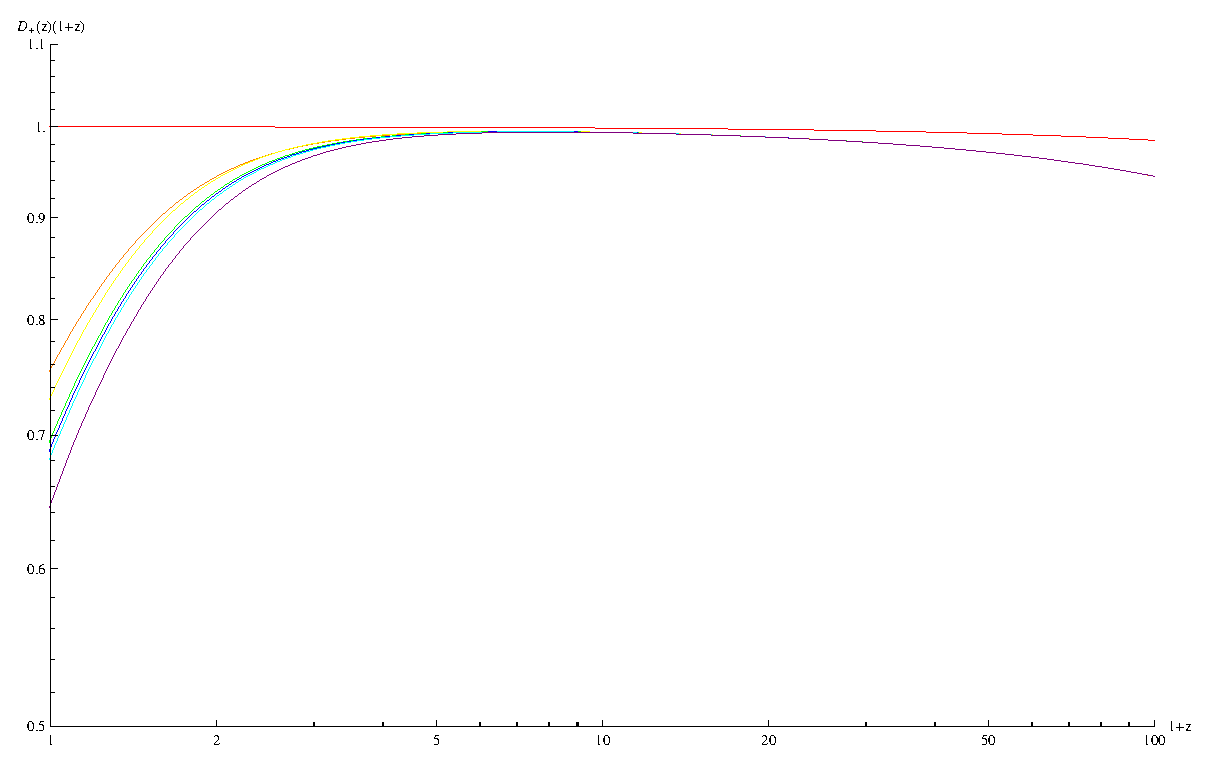
\includegraphics[width=400pt]{CPL_GrowthFactors.eps}
\caption{The growth factors of different models including sCDM, LCDM and five other CPL parameterised dark energy model}\label{fig:CPL_GrowthFactors}
\end{figure}



\begin{figure}[!htbp]
\centering
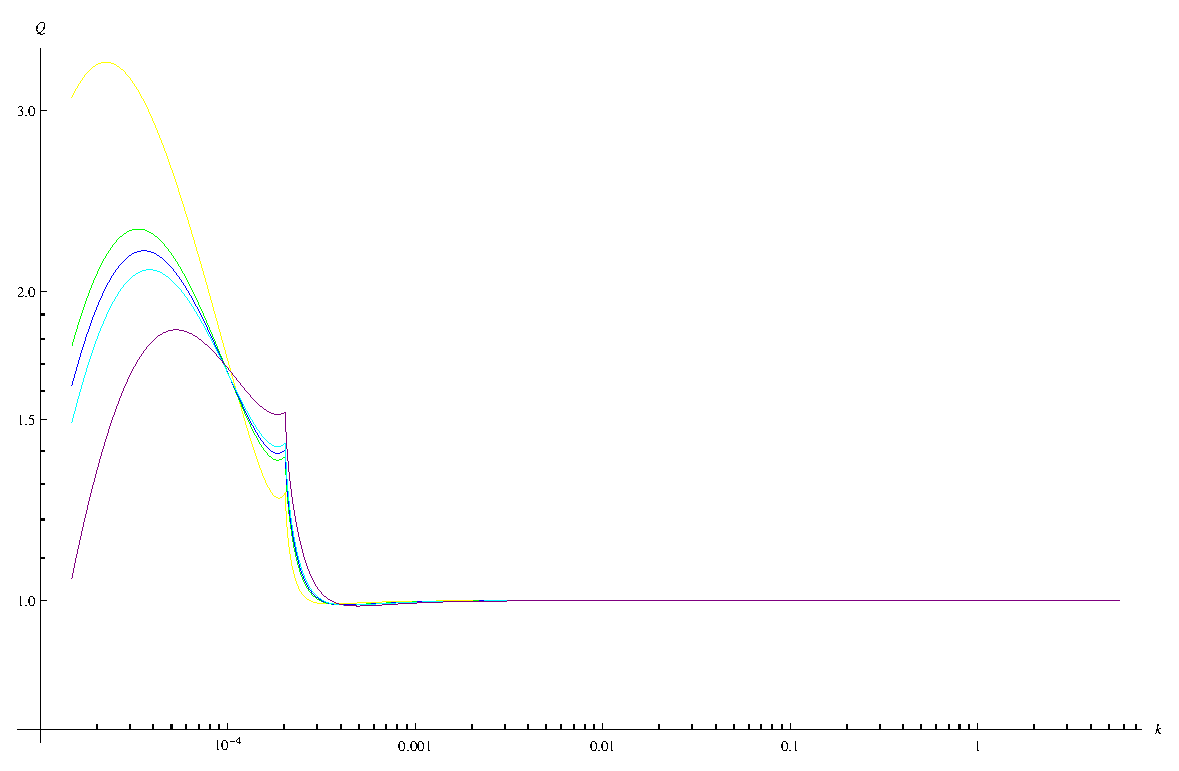
\includegraphics[width=400pt]{CPL_QFactors.eps}
\caption{The Q factors of different models including sCDM, LCDM and five other CPL parameterised dark energy model}\label{fig:CPL_QFactors}
\end{figure}





\begin{figure}[!htbp]
\centering
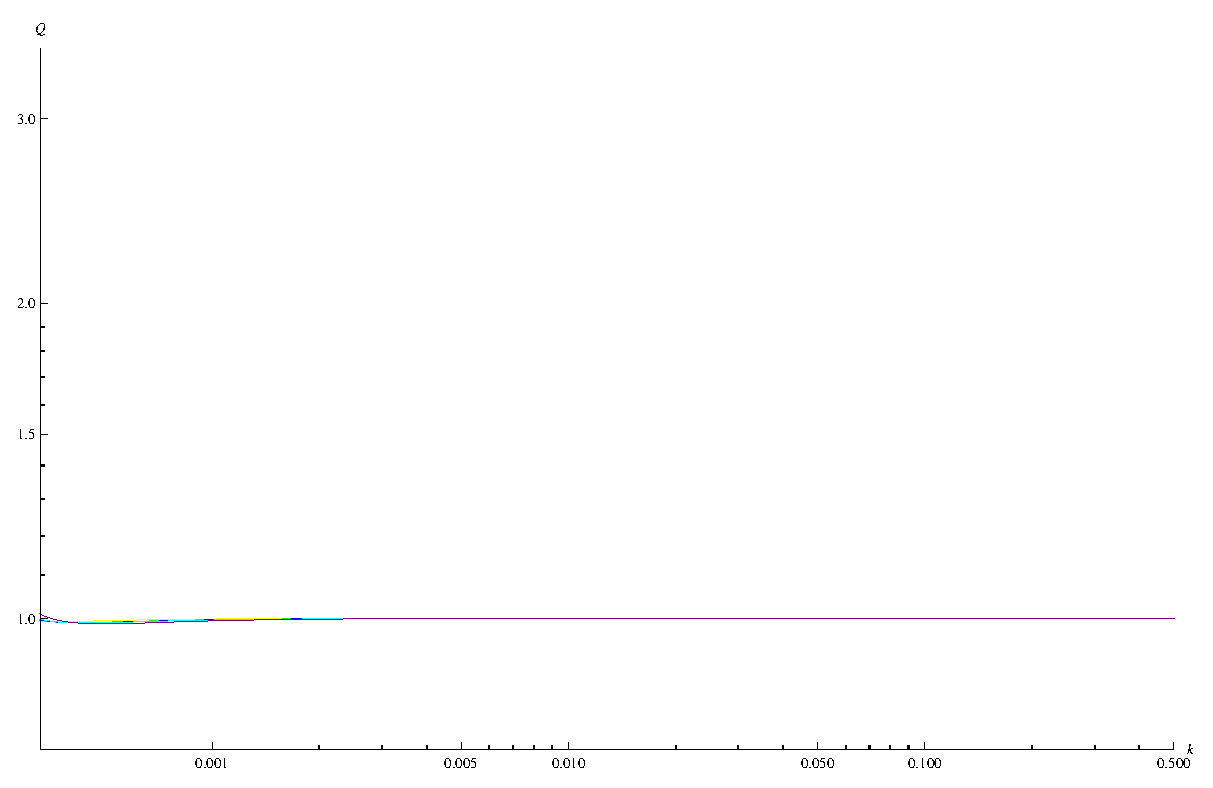
\includegraphics[width=400pt]{CPL_QFactors_Cut.eps}
\caption{The Q factors (within a range) of different models including sCDM, LCDM and five other CPL parameterised dark energy model}\label{fig:CPL_QFactors_Cut}
\end{figure}

Figure \ref{fig:CPL_GrowthFactors} has peaks. These peaks comes from the $1+z<1$ part of the growth factor. These should be cut off latter.

The figures show the smaller the parameters $w_a$, the larger deviation from LCDM at late times.




\begin{figure}[!htbp]
\centering
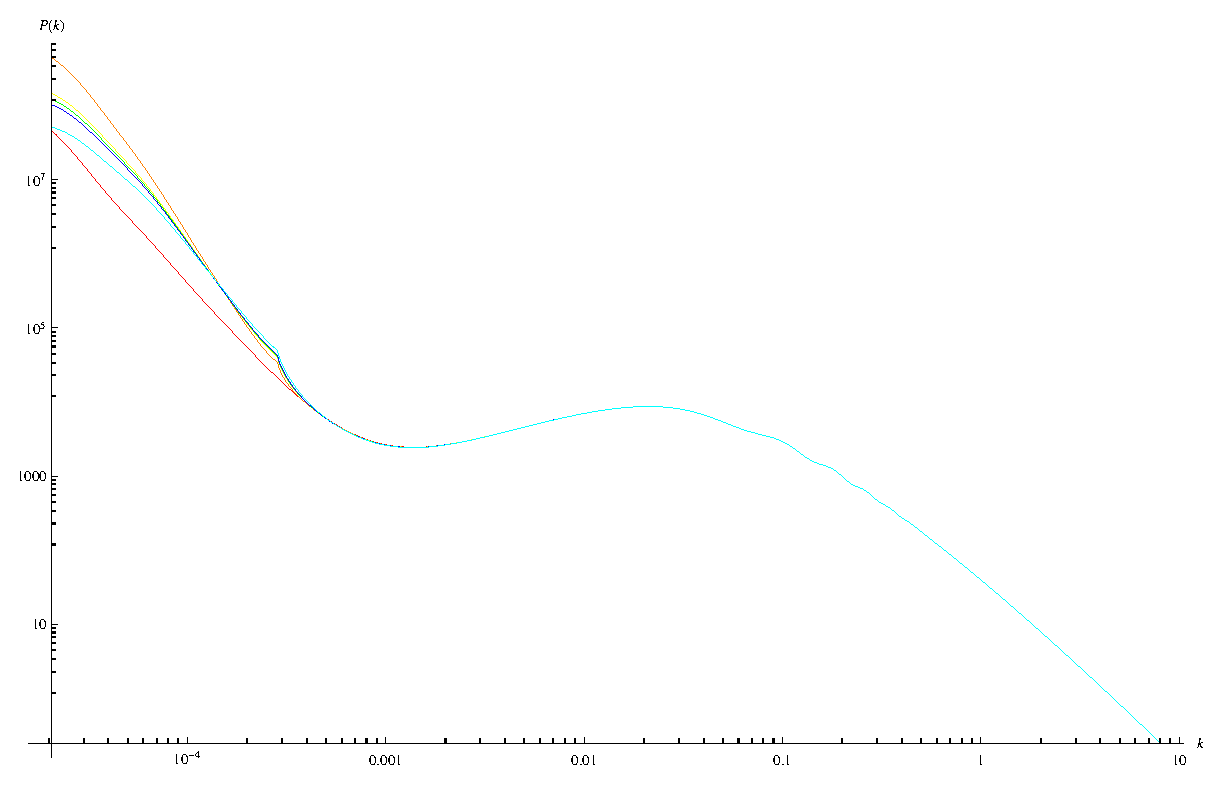
\includegraphics[width=400pt]{CPL_PowerSpectrums.eps}
\caption{The power spectrums of different models including sCDM, LCDM and five other CPL parameterised dark energy model}\label{fig:CPL_PowerSpectrums}
\end{figure}





\begin{figure}[!htbp]
\centering
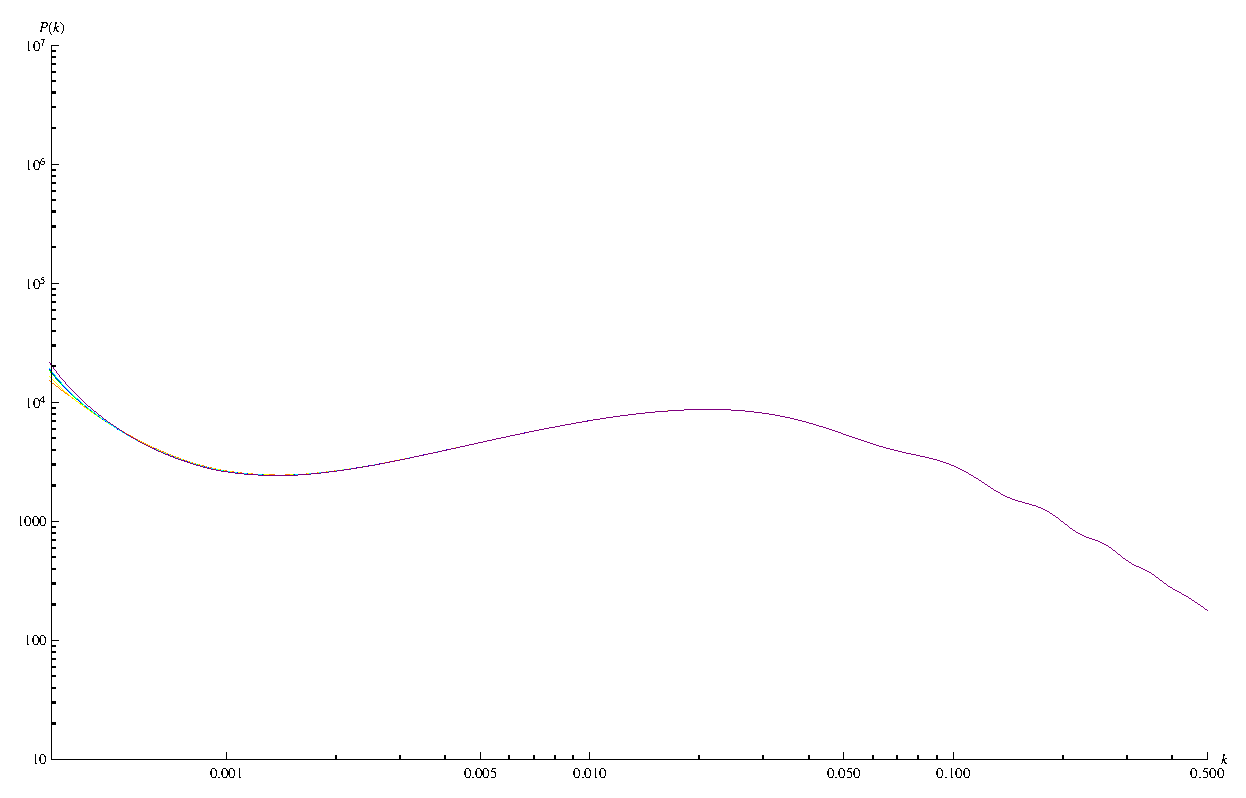
\includegraphics[width=400pt]{CPL_PowerSpectrums_Cut.eps}
\caption{The power spectrums (within a range) of different models including sCDM, LCDM and five other CPL parameterised dark energy model}\label{fig:CPL_PowerSpectrums_Cut}
\end{figure}





Figure \ref{fig:CPL_PowerSpectrums_Cut} shows that the power spectrum can hardly be recognised until today. (I am making too small changes in the parameters. More references needed here in order make this clear.)








\subsection{\color{blue}First Supplements}


\begin{quotation}
{\color{blue}


\begin{enumerate}

\item\label{item:HubbleDistance}

\begin{figure}[!htpb]
\centering
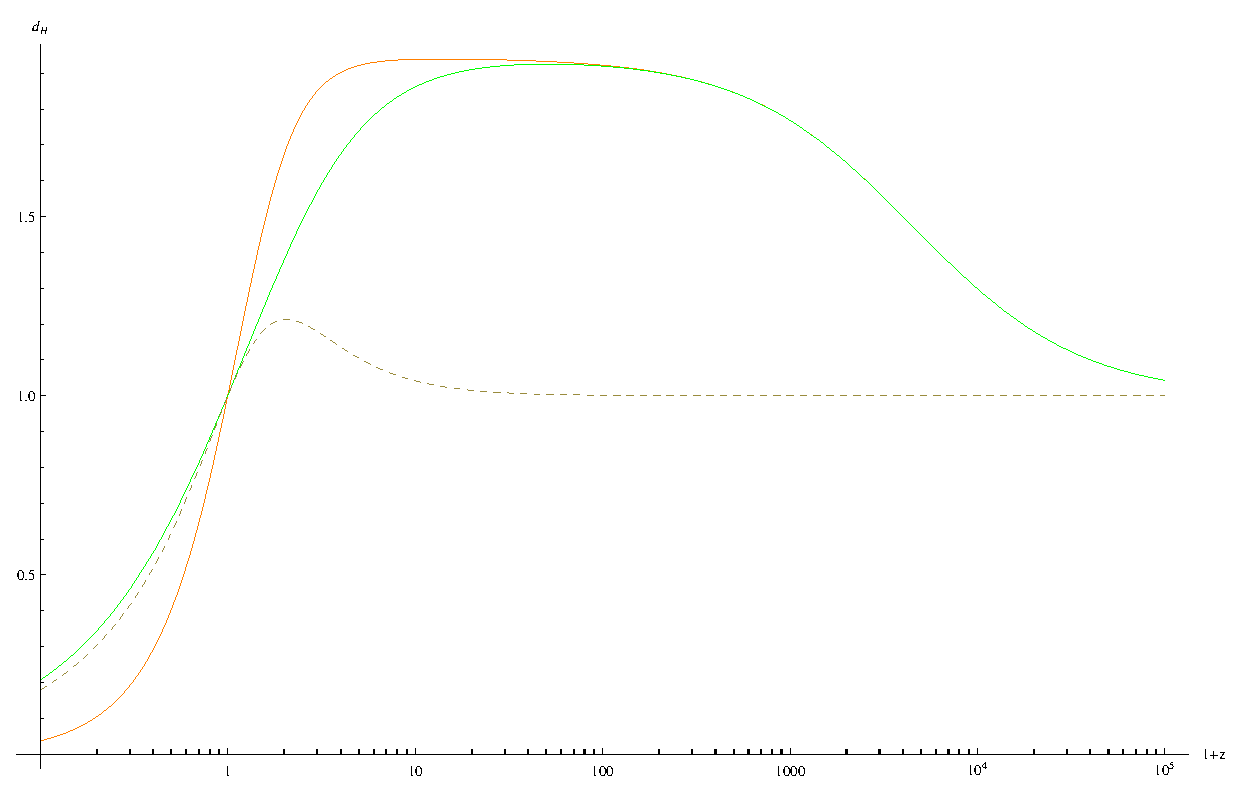
\includegraphics[width=350pt]{DE_Supp_HubbleDistances.eps}
\caption{\color{blue}Hubble distance. Dashed line is the Hubble distance ratio of DE (with $w=-0.5$) and LCMD.}\label{fig:DE_Supp_HubbleDistances}
\end{figure}

Figure \ref{fig:DE_Supp_HubbleDistances} corresponds to Figure 1 {a} in Fernando's. I think $1+z<1$ is of nonsense because redshift $z$ should be larger than 1 if we only care about the present and the past. So I only plotted the $1+z>1$. Here my figure is different from Fernando's at about $1+z<10$. All the lines converge at $z=0$ in my plot because all the Hubble functions becomes the Hubble constant of today at that redshift. I have no idea why Fernando's plot do not. (And I have no idea why he plotted $z<0$).


\item
As said in the previous item, redshift less than zero is not so usefull.

\item
I have already check the effect of $\Omega_{m0}$ and $\Omega_{de0}$. The figure does not change very much.

\begin{figure}[!htpb]
\centering
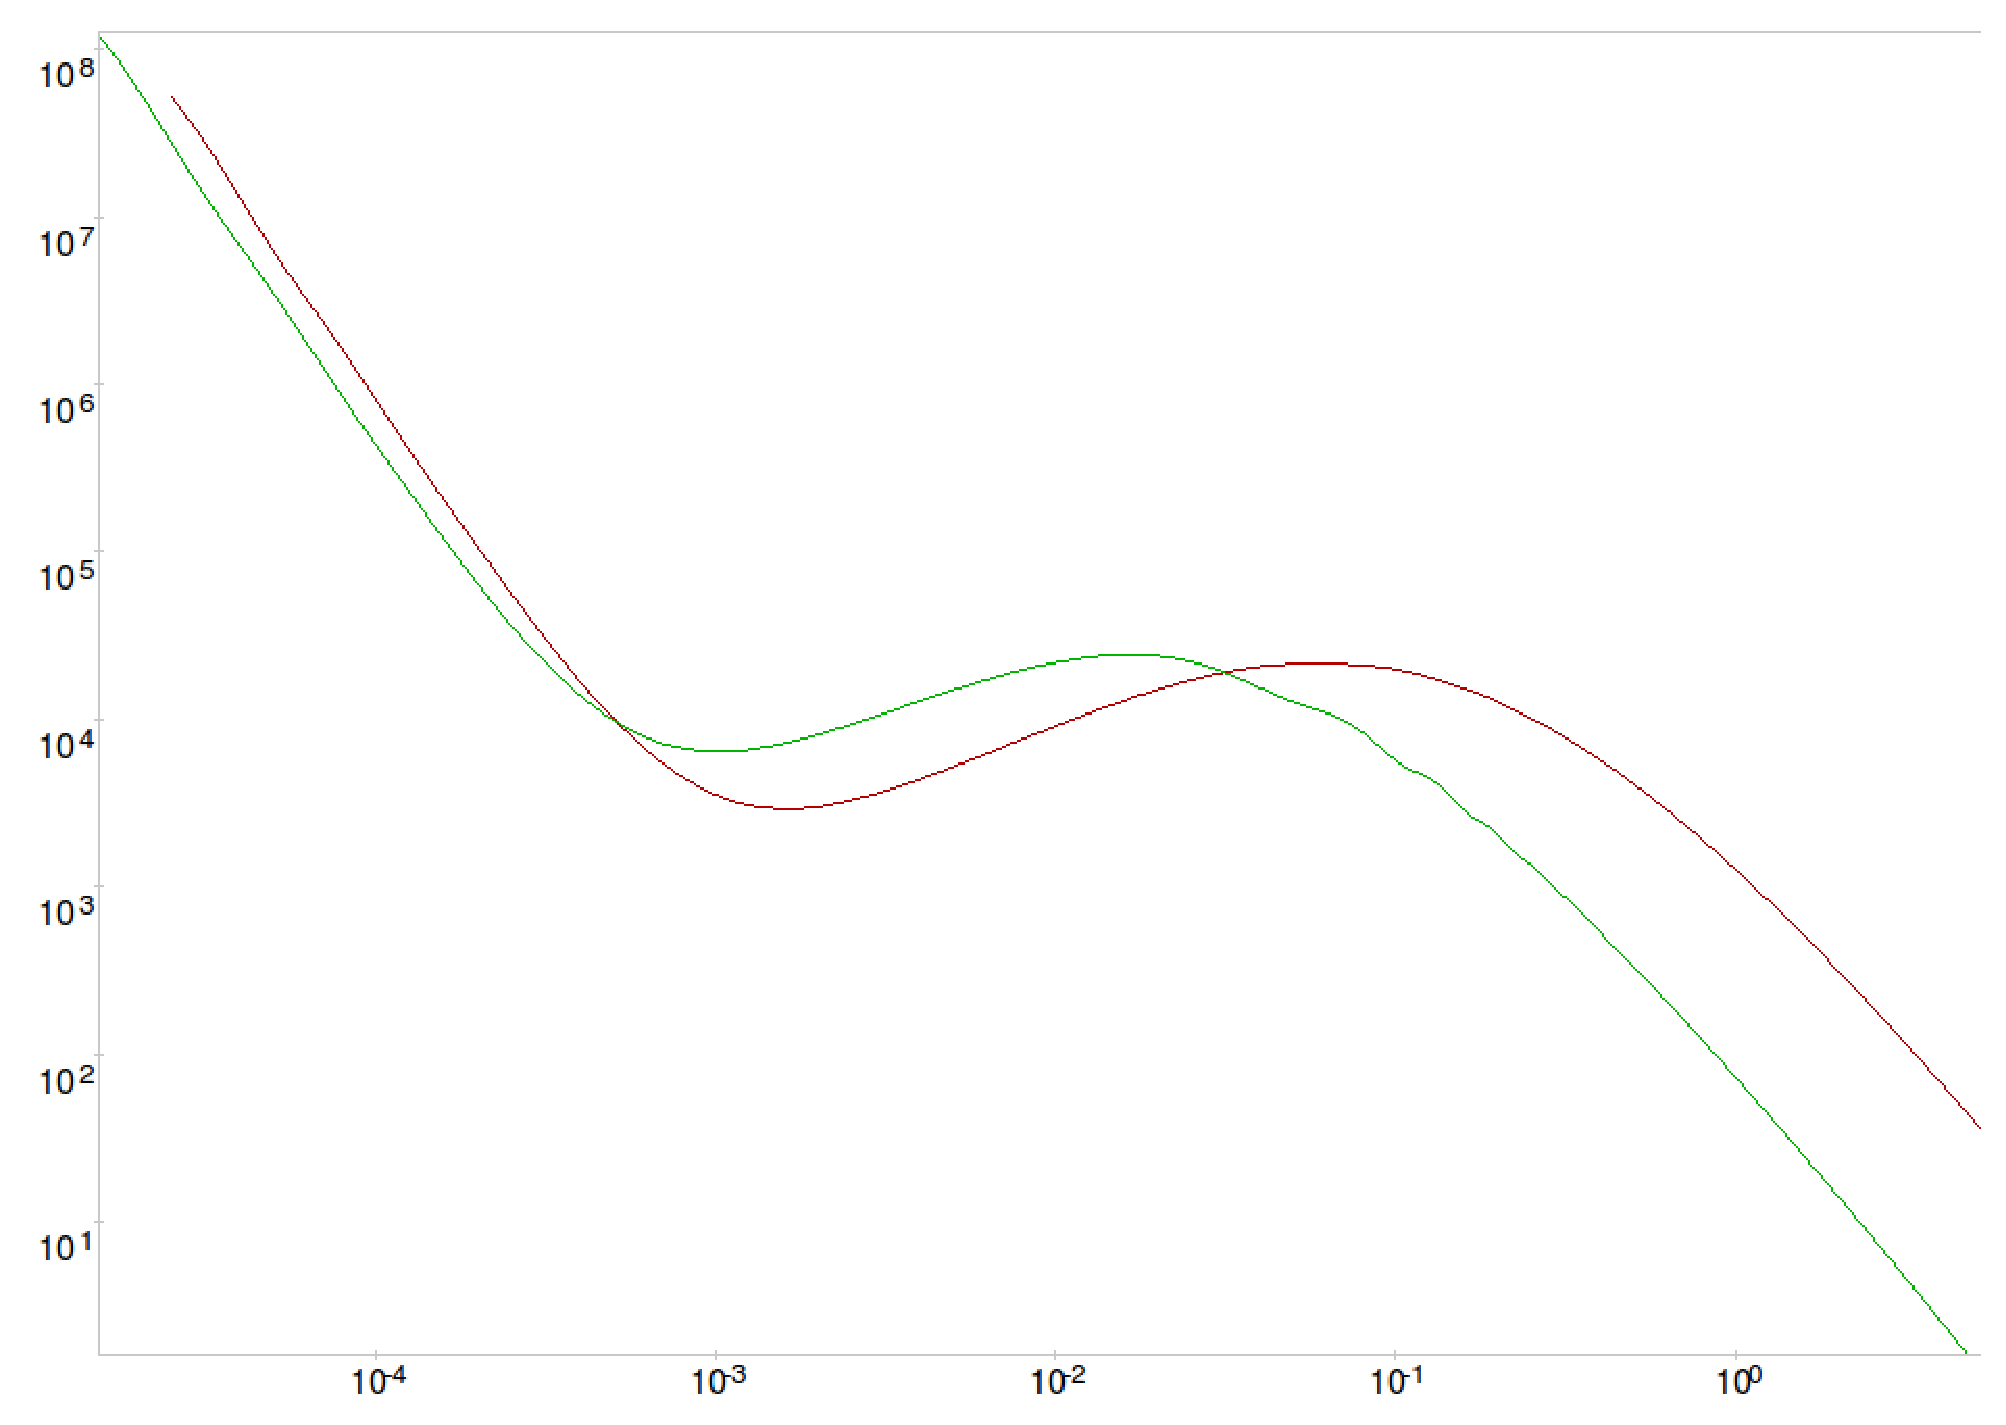
\includegraphics[width=350pt]{PowerSpectrumDEsCDMCMBEASY.eps}
\caption{\color{blue}Power spectrum of dark energy model with $\Omega_{DE0}=0$ and $\Omega_{DE0}=0.7$. The red line is the sCDM model.}
\end{figure}

That's why I did not plot figure varying in $\Omega_{DE0}$.

\item
I think there is no need to plot figures on different DE and DM abundances. Is there anything to be expected from plotting these figures?

Small $k$ corresponds to negative redshift.

\item


\begin{figure}[!htpb]
\centering
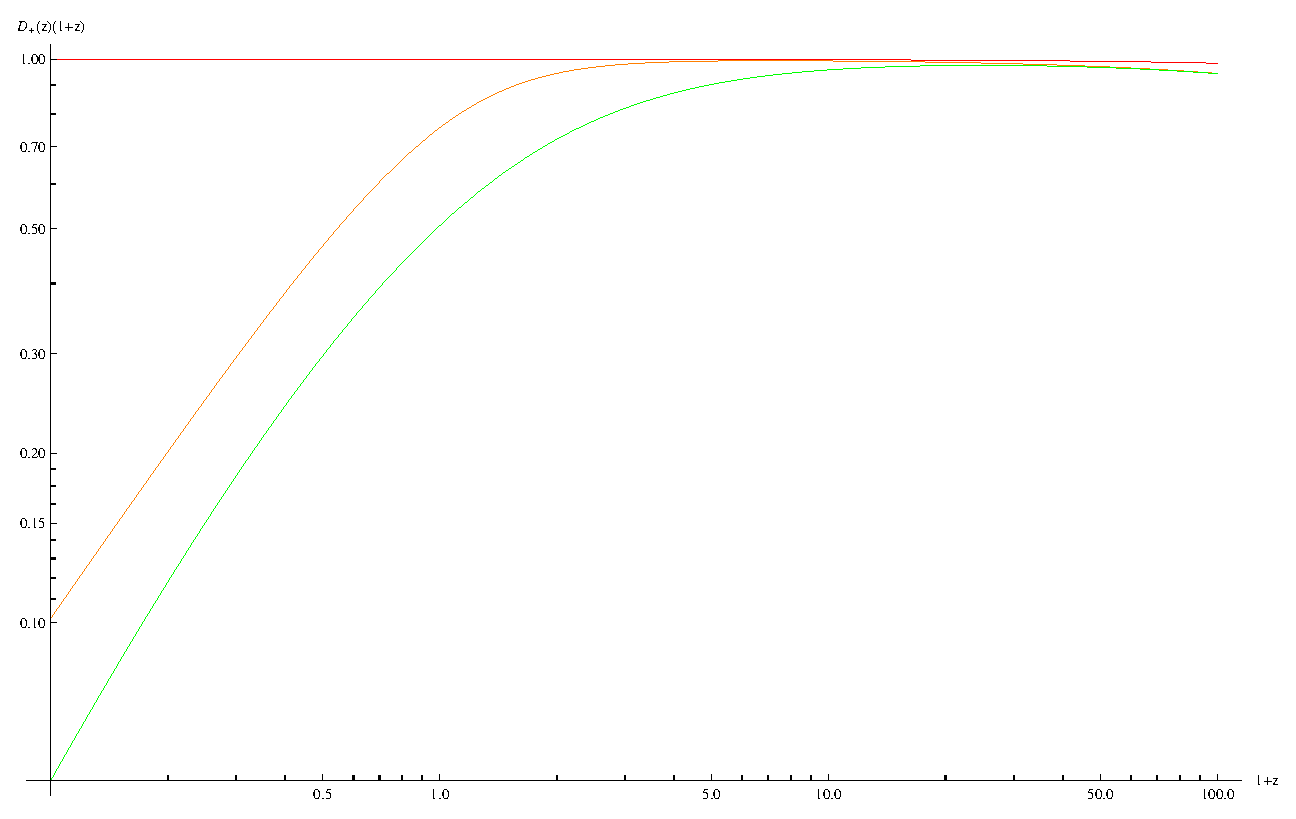
\includegraphics[width=350pt]{DE_Supp_GrowthFactors.eps}
\caption{\color{blue}Growth factors are given in this figure. Dashed line is the Hubble distance ratio of DE (with $w=-0.5$) and LCMD.}\label{fig:DE_Supp_GrowthFactors}
\end{figure}

The growth factors in figure \ref{fig:DE_Supp_GrowthFactors} is plotted within $1+z\sim[0.1,1000]$. As argued in \ref{item:HubbleDistance}, the data is useless when $z<0$ unless one is going to check the future evolution of the universe.
{\bf That is why I give two figures for one quantity sometimes: one for a larger range and one for a suitable range.}



\item

The CPL EoS used here is $w=w_0+w_a(1-a)$. The paramters chosen are listed in the table below.

\vspace{2ex}
\begin{center}
\begin{tabular}{|c|c|}\hline
{\bf Color} & {\bf Model} \\\hline
Red & sCDM \\\hline
Orange & LCDM \\\hline
Yellow & $w_0=-1$ \& $w_a=0.1$ \\ \hline
Green &  $w_0=-1$ \& $w_a=-0.1$ \\ \hline
Blue & $w_0=-0.9$ \& $w_a=-0.1$ \\ \hline
Cyan & $w_0=-0.9$ \& $w_a=0.1$ \\ \hline
Purple & $w_0=-0.9$ \& $w_a=-0.2$ \\ \hline
\end{tabular}
\end{center}
\vspace{2ex}


\begin{figure}[!htpb]
\centering
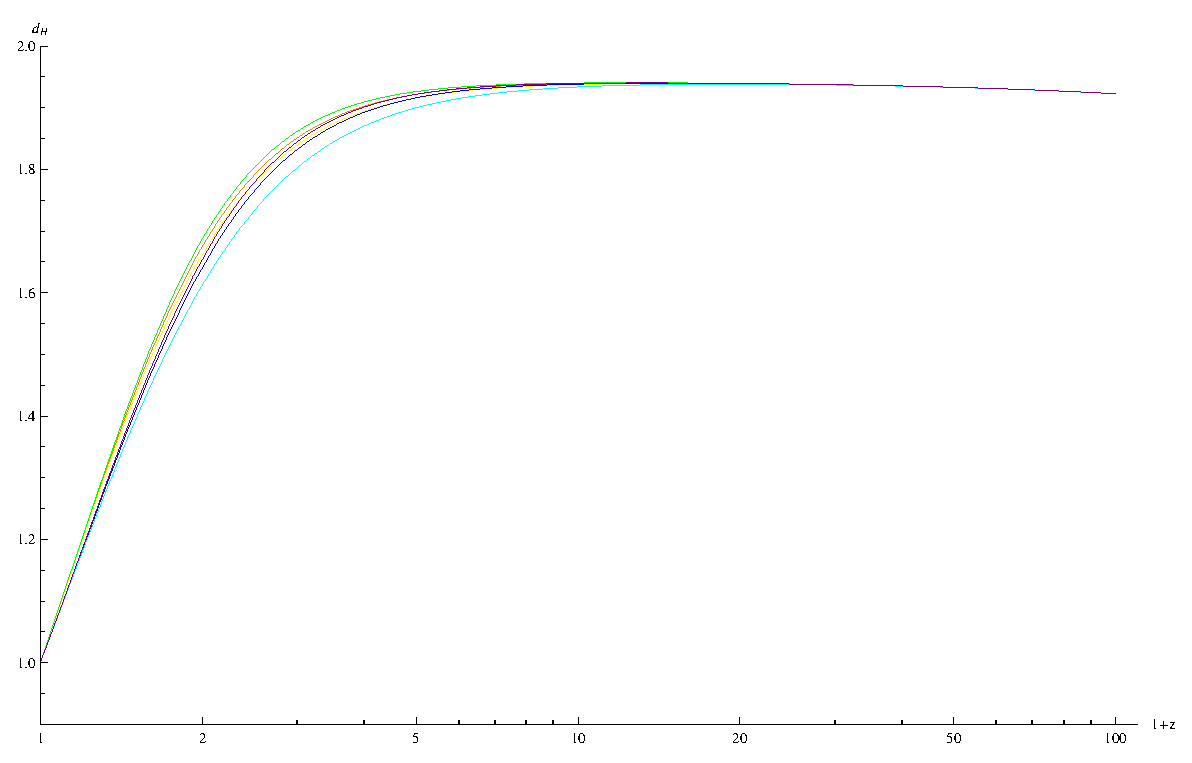
\includegraphics[width=350pt]{CPL_Supp_HubbleDistances.eps}
\caption{\color{blue}Hubble distance of CPL dark energy.}\label{fig:CPL_Supp_HubbleDistances}
\end{figure}

\begin{figure}[!htpb]
\centering
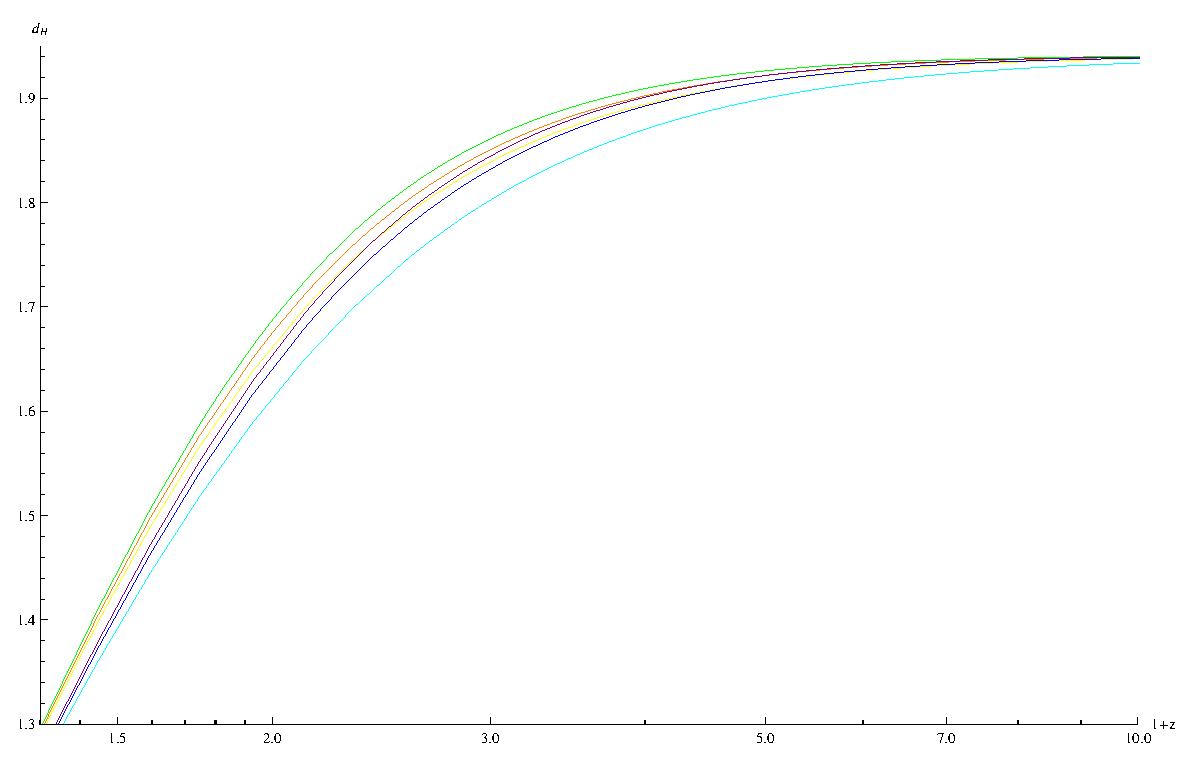
\includegraphics[width=350pt]{CPL_Supp_HubbleDistances_Cut.eps}
\caption{\color{blue}Hubble distance of CPL dark energy.}\label{fig:CPL_Supp_HubbleDistances_Cut}
\end{figure}

\begin{figure}[!htpb]
\centering
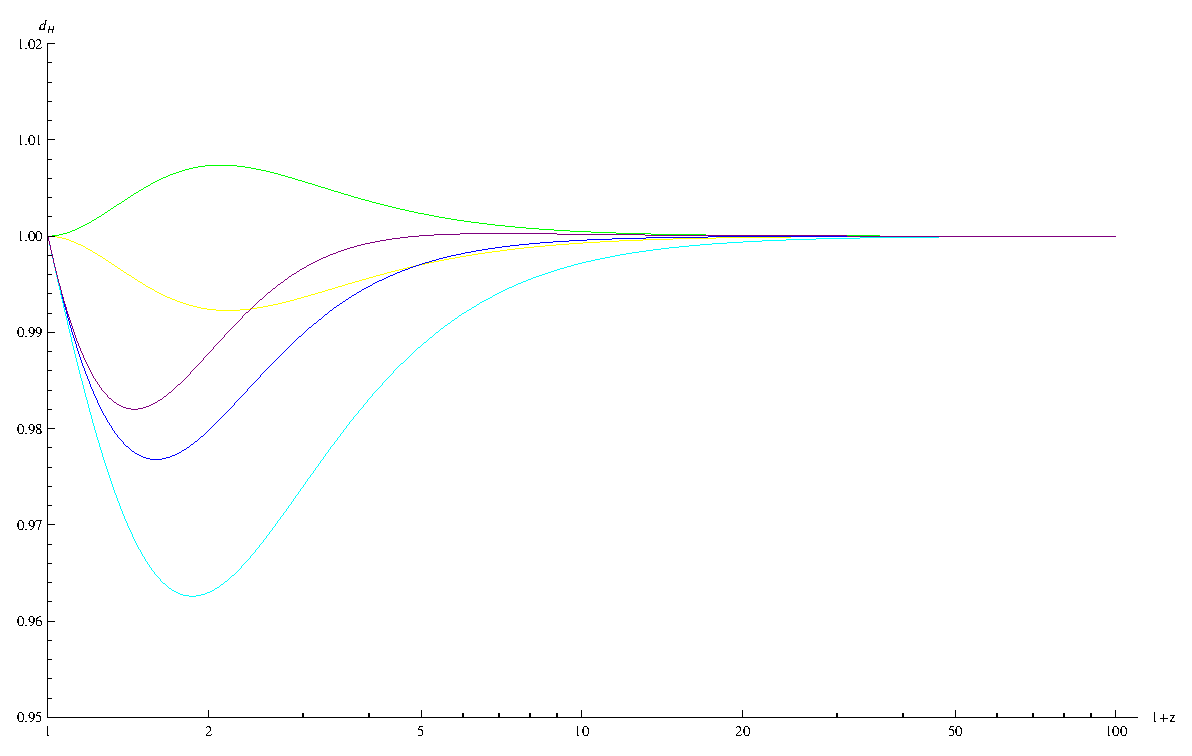
\includegraphics[width=350pt]{CPL_Supp_HubbleDistances_DivideLCDM.eps}
\caption{\color{blue}Hubble distance of CPL dark energy in units of LCDM Hubble distances at the corresponding value.}\label{fig:CPL_Supp_HubbleDistances_DivideLCDM}
\end{figure}

\begin{figure}[!htpb]
\centering
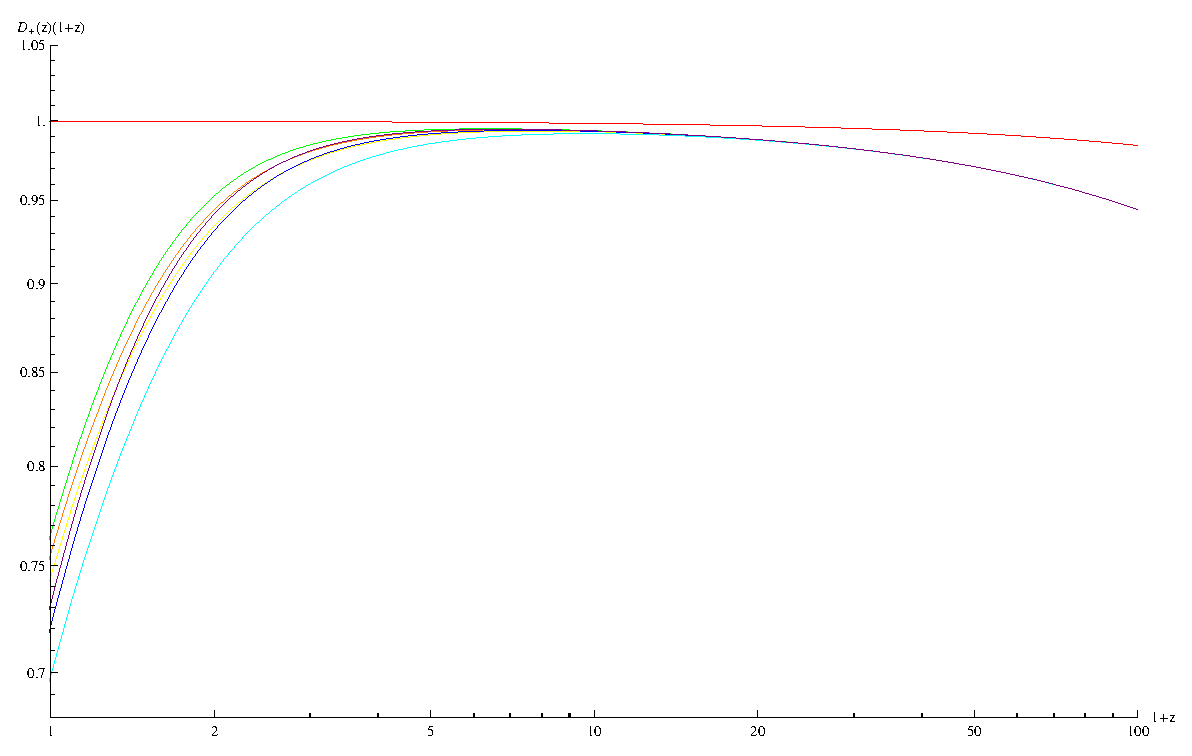
\includegraphics[width=350pt]{CPL_Supp_GrowthFactors.eps}
\caption{\color{blue}Growth factors of CPL dark energy and LCDM in units of sCDM.}\label{fig:CPL_Supp_GrowthFactors}
\end{figure}

\begin{figure}[!htpb]
\centering
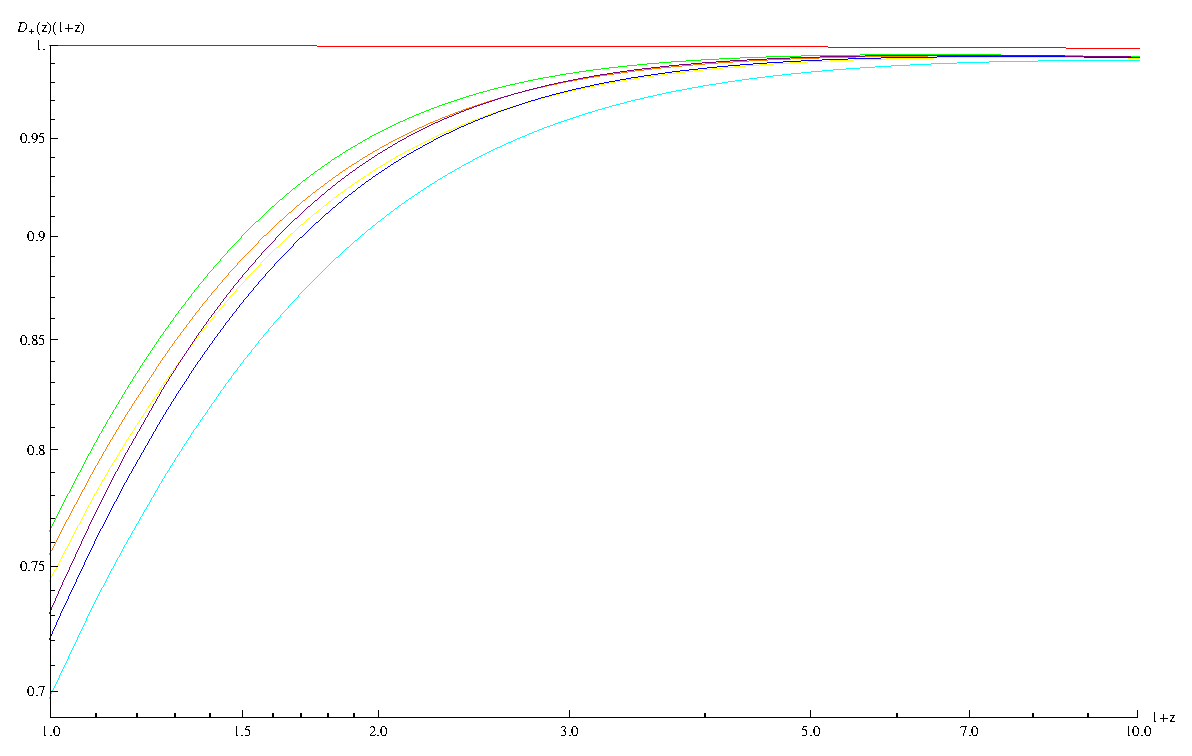
\includegraphics[width=350pt]{CPL_Supp_GrowthFactors_Cut.eps}
\caption{\color{blue}Growth factors of CPL dark energy and LCDM in units of sCDM.}\label{fig:CPL_Supp_GrowthFactors_Cut}
\end{figure}




\begin{figure}[!htpb]
\centering
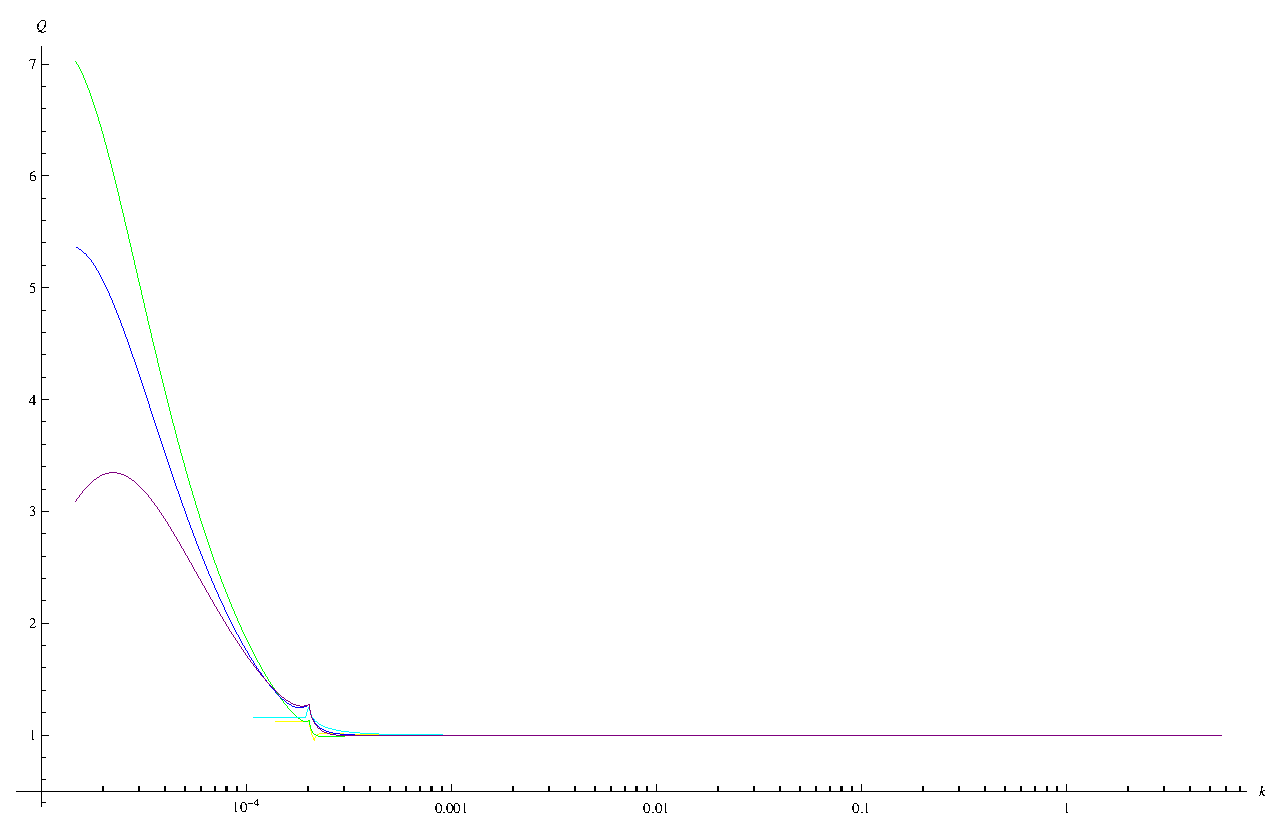
\includegraphics[width=350pt]{CPL_Supp_QFactors.eps}
\caption{\color{blue}Q factors of CPL dark energy and LCDM in units of sCDM.}\label{fig:CPL_Supp_QFactors}
\end{figure}


\begin{figure}[!htpb]
\centering
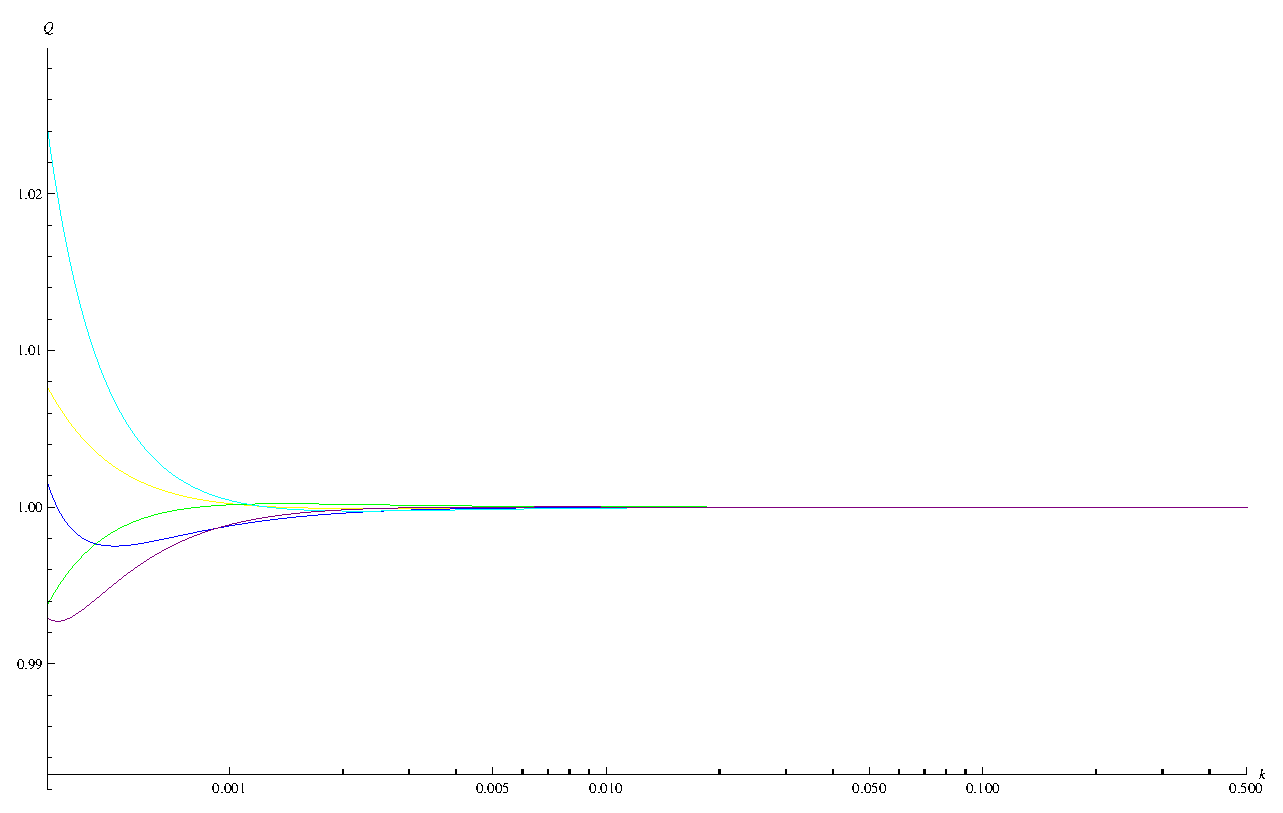
\includegraphics[width=350pt]{CPL_Supp_QFactors_Cut.eps}
\caption{\color{blue}Q factors of CPL dark energy and LCDM in units of sCDM.}\label{fig:CPL_Supp_QFactors_Cut}
\end{figure}

\begin{figure}[!htpb]
\centering
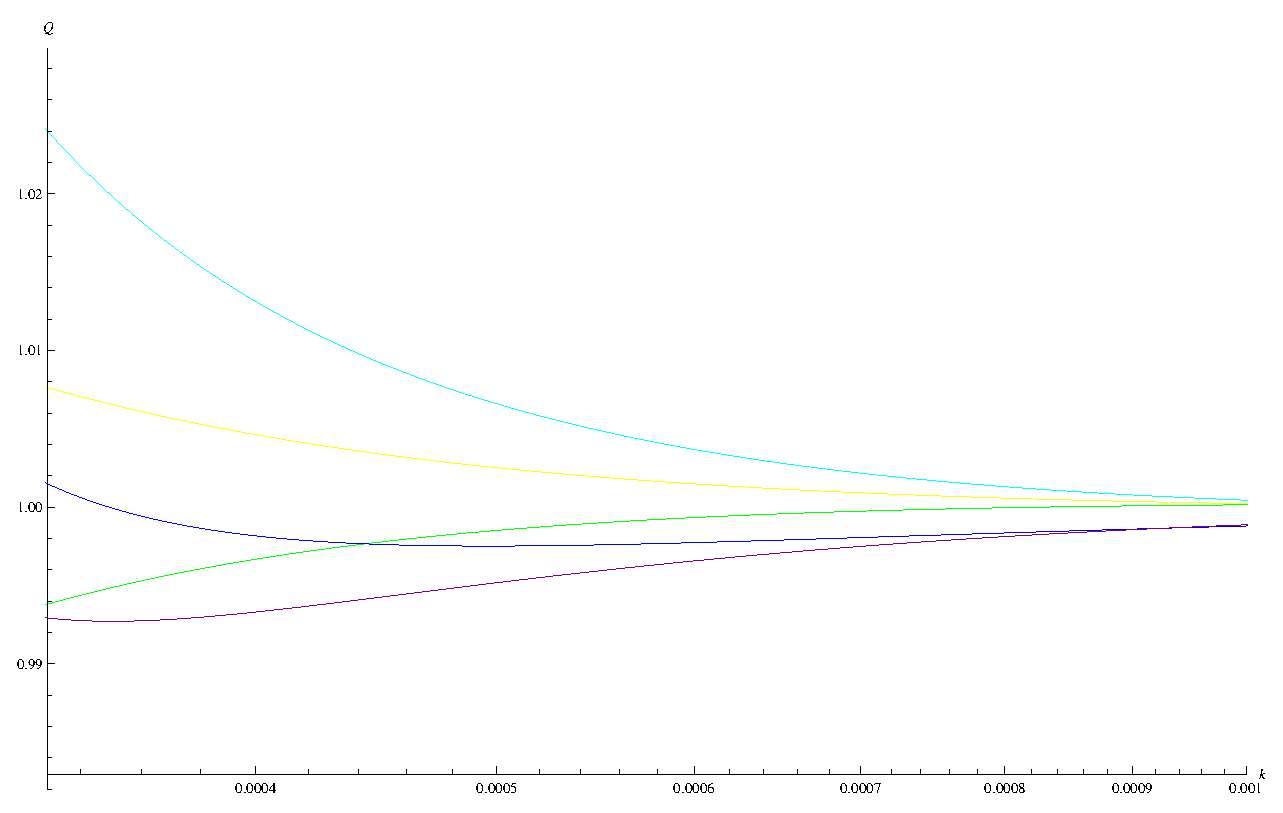
\includegraphics[width=350pt]{CPL_Supp_QFactors_Detail.eps}
\caption{\color{blue}Q factors of CPL dark energy and LCDM in units of sCDM.}\label{fig:CPL_Supp_QFactors_Detail}
\end{figure}


\begin{figure}[!htpb]
\centering
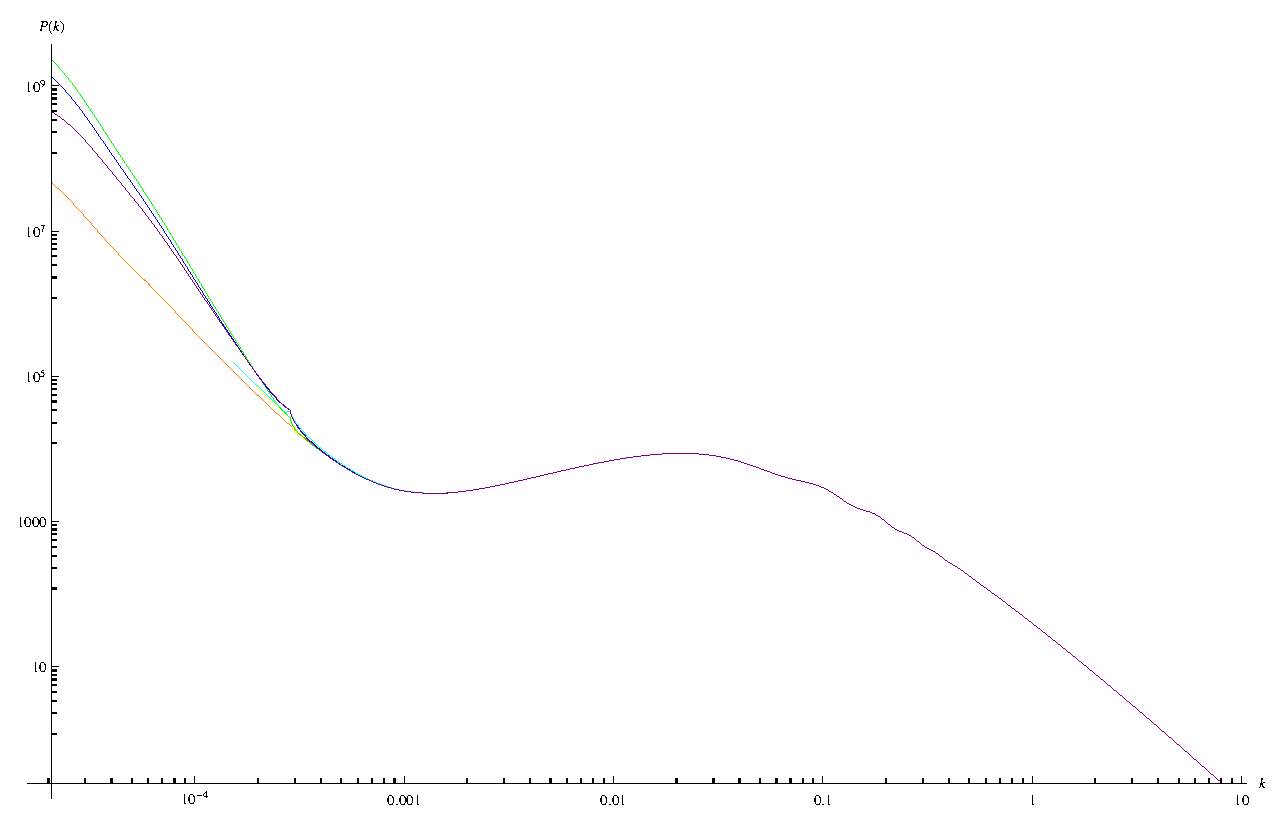
\includegraphics[width=350pt]{CPL_Supp_PowerSpectrums.eps}
\caption{\color{blue}Power spectrum of CPL dark energy and LCDM in units of sCDM.}\label{fig:CPL_Supp_PowerSpectrums}
\end{figure}


\begin{figure}[!htpb]
\centering
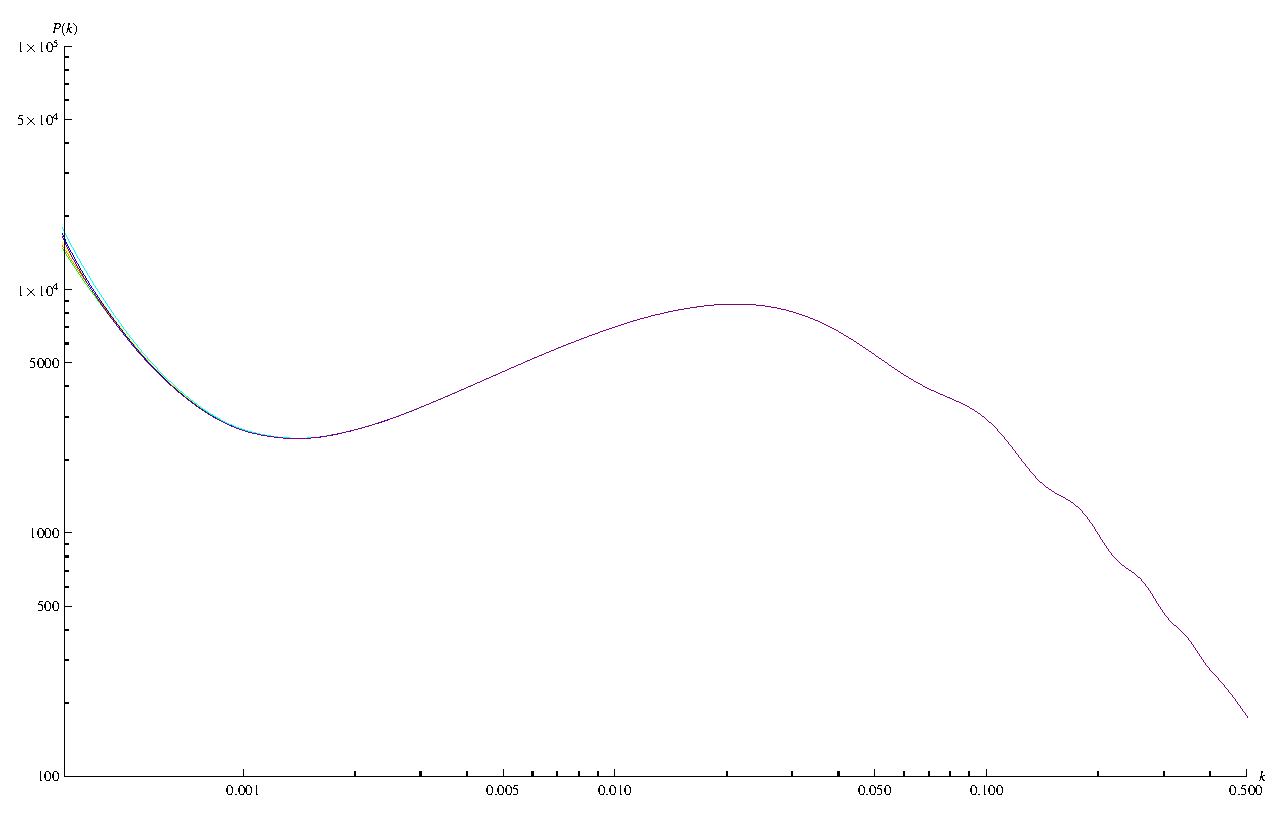
\includegraphics[width=350pt]{CPL_Supp_PowerSpectrums_Cut.eps}
\caption{\color{blue}Power spectrum of CPL dark energy and LCDM in units of sCDM.}\label{fig:CPL_Supp_PowerSpectrums_Cut}
\end{figure}


\begin{figure}[!htpb]
\centering
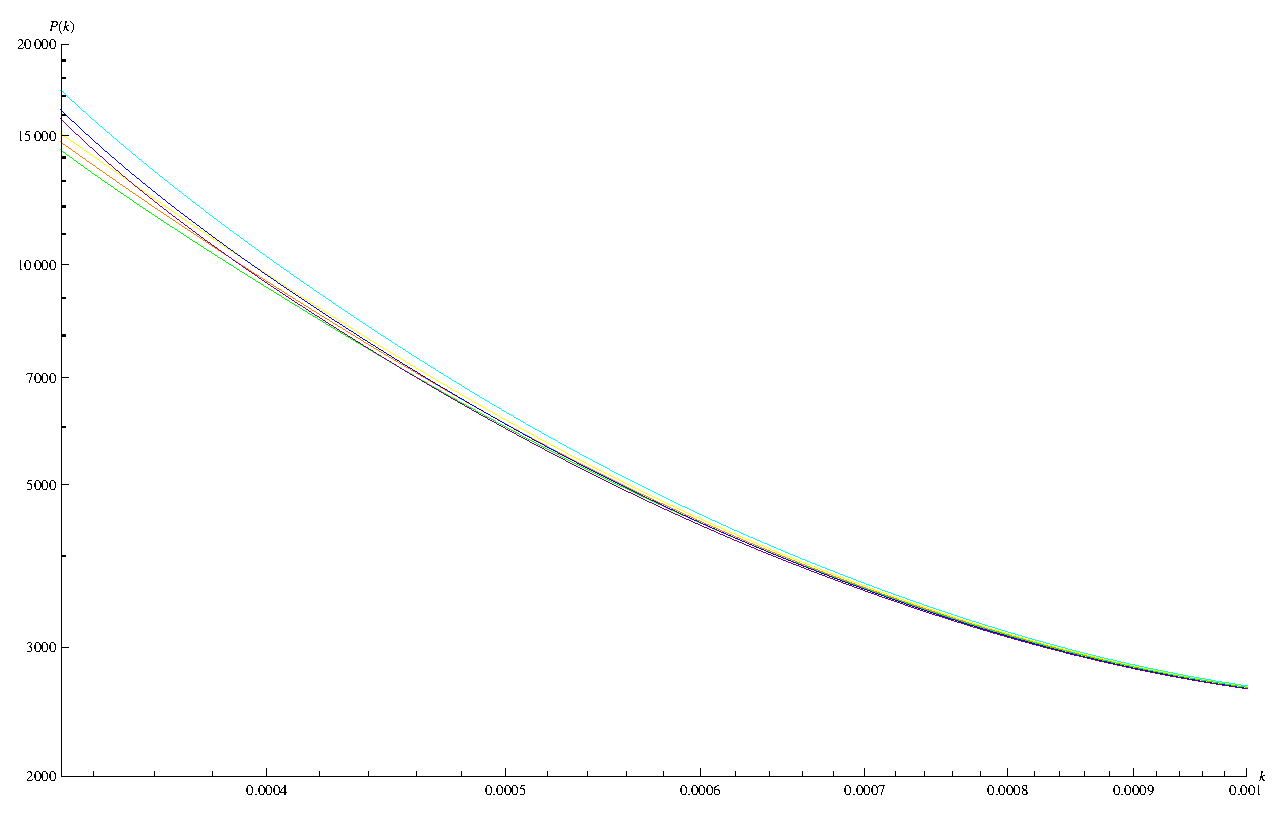
\includegraphics[width=350pt]{CPL_Supp_PowerSpectrums_Detail.eps}
\caption{\color{blue}Power spectrum of CPL dark energy and LCDM in units of sCDM.}\label{fig:CPL_Supp_PowerSpectrums_Detail}
\end{figure}

The parameters chosen only have effects on small redshift. This is because the parameters all satisfy the condition that $w_0\rightarrow -1$ and $w_a\rightarrow 0$.

By comparing yellow line ($w_0=-1, w_a=0.1$) and green line ($w_0=-1, w_a=-0.1$), we can see positive $w_a$ leads to a larger then LCDM Hubble distance when $w_0=-1$. This is in accord with the series form of Hubble equation \ref{eq:CPL_HubbleEquation_Series} since $w_0=-1$ eliminates the first order term and the $w_a$ determines whether the expression is larger then one.
Other comparisons like green line and blue line, blue line and purple line in Figure \ref{fig:CPL_Supp_HubbleDistances} \ref{fig:CPL_Supp_HubbleDistances_Cut} \ref{fig:CPL_Supp_HubbleDistances_DivideLCDM} can also be interpreted by equation \ref{eq:CPL_HubbleEquation_Series}.


Growth factors are also following the expansion. Cyan line ($w_0=-0.9, w_a=0.1$) has smaller Hubble distances that others at late time, so the growth drops since growth factor is positively correlated to the size of the Hubble distance. The changes in growth factors when changing the parameters are exactly positively correlated to the size of Hubble distance changes. For example, the yellow line ($w_0=-1, w_a=0.1$) crosses the purple line ($w_0=-0.9, w_a=-0.2$) in figure \ref{fig:CPL_Supp_GrowthFactors} \ref{fig:CPL_Supp_GrowthFactors_Cut} as they cross each other in the figure of Hubble distance.

Figure \ref{fig:CPL_Supp_QFactors} has a region $k<3.3 * 10^{-4}$ that is corresponding to scale factor $a>1$. So I give another two plots figure \ref{fig:CPL_Supp_QFactors_Cut} and \ref{fig:CPL_Supp_QFactors_Detail}. The same thing is done for power spectrum.

The power spectrum is consistent with the Hubble distance figure: larger Hubble distance generates weaker power.




\item
Because we are using adiabatic initial conditions with a form $P\sim \frac{1}{k^3}$.

At $a\sim 10^{-3}$ and $a\sim 1$, we have $k\sim 1$ and $k\sim 10^{-3}$ correspondingly. The growth factor with amplifies the initial perturbation by about $10^3$ to get the current value $P\sim 10^6$ for $k\sim 1$ and the current value is $10^9$ for initial perturbation at $a\sim 1$ (or $k\sim 10^{-3}$) since it has not evolved. This simple calculation show the shape of power spectrum is definitely going up at small k.

item
As stated previously, the inconsistent part is $z<0$, so there is no need to worry about.





\end{enumerate}



}
\end{quotation}







%%%%%%%%%%%%%%%%%%%%%%%%%%%%%%%%%%%%%%%%%%%%%%%%%%%%%%%%%
%%%%%%%%%%%%%%%%%%%%%%%%%%%%%%%%%%%%%%%%%%%%%%%%%%%%%%%
%%%%%%%%%%%%%%%%%%%%%%%%%%%%%%%%%%%%%%%%%%%%%%%%%%%%%%%%
%%%%%%%%%%%%%%%%%%%%%%%%%%%%%%%%%%%%%%%%%%%%%%%%%%%%%%%
%%%%%%%%%%%%%%%%%%%%%%%%%%%%%%%%%%%%%%%%%%%%%%%%%%%%%%%
\end{document}